% -*- coding: UTF-8 -*-
\documentclass{article}
\usepackage{amsmath}
\usepackage{tikz}

\begin{document}
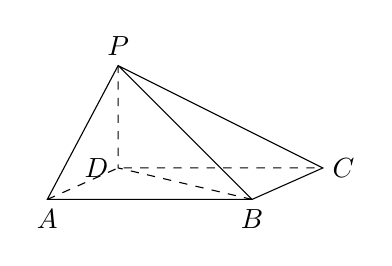
\begin{tikzpicture}

  \coordinate[label=-90:$A$] (a) at (0,0);
  \coordinate[label=-90:$B$] (b) at (2.6,0);
  \coordinate[label=0:$C$] (c) at (3.5,0.4);
  \coordinate[label=180:$D$] (d) at (0.9,0.4);
  \coordinate[label=90:$P$] (p) at (0.9,1.7);

  \draw (p) -- (a) -- (b) -- (c)  -- cycle -- (b);
  \draw[dashed] (a) -- (d) -- (c)  (b) -- (d) -- (p);

\end{tikzpicture}
\end{document}
